\documentclass[20pt, a0paper, landscape]{tikzposter}
% \usepackage[utf8]{inputenc}
 
\title{OPTIMAL FISHING RATES FOR MULTIPLE FLEETS}
\author{Steven Martell and Catarina Wor}
\date{\today}
\institute{INTERNATIONAL PACIFIC HALIBUT COMMISSION}
 
\usepackage{blindtext}
\usepackage{comment}

% Themes
\usetheme{Default} 
\usetheme{Rays} 
% \usetheme{Basic} 
% \usetheme{Simple} 
% \usetheme{Envelope} 
% \usetheme{Wave} 
% \usetheme{Board} 
% \usetheme{Autumn} 
% \usetheme{Desert} 


% Block styles
\useblockstyle{Default}
\useblockstyle{Basic}
\useblockstyle{Minimal}
\useblockstyle{Envelope}
\useblockstyle{Corner}
\useblockstyle{Slide} 
\useblockstyle{TornOut}

% Note styles
\usenotestyle{Sticky}


% Note colors
\definecolor{notefgcolor}{named}{black}
\definecolor{notebgcolor}{HTML}{FCF0AD}



% additional packages
% \usepackage{times}
\usepackage{amsmath,amsthm, amssymb, latexsym, bm}
% \usepackage{exscale}
% \usepackage{ragged2e}
% \boldmath
% \usepackage{booktabs, array}
% \usepackage{rotating} %sideways environment
\usepackage[english]{babel}
\usepackage[latin1]{inputenc}
% \listfiles
% \graphicspath{{figures/}}
% \graphicspath{{FIGS/}}




% abbreviations
\usepackage{xspace}
\makeatletter
\DeclareRobustCommand\onedot{\futurelet\@let@token\@onedot}
\def\@onedot{\ifx\@let@token.\else.\null\fi\xspace}
\def\eg{{e.g}\onedot} \def\Eg{{E.g}\onedot}
\def\ie{{i.e}\onedot} \def\Ie{{I.e}\onedot}
\def\cf{{c.f}\onedot} \def\Cf{{C.f}\onedot}
\def\etc{{etc}\onedot}
\def\vs{{vs}\onedot}
\def\wrt{w.r.t\onedot}
\def\dof{d.o.f\onedot}
\def\etal{{et al}\onedot}
\makeatother

\newcommand{\fspr}{F$_{\rm{SPR=35\%}}$}
\newcommand{\bspr}{B$_{\rm{SPR=35\%}}$}
\newcommand{\rspr}{R$_{\rm{SPR=35\%}}$}
\newcommand{\fofl}{F$_{\rm{OFL}}$}

\usepackage{pifont}% http://ctan.org/pkg/pifont
\newcommand{\cmark}{\ding{51}}%
\newcommand{\xmark}{\ding{55}}%

\newcommand{\fmsy} {F$_{\rm{\textbf{MSY}}}$}

\newcommand{\dye}  { \dfrac{{\partial y_k}}{{\partial f_k}} }%
\newcommand{\dre}  { \dfrac{{\partial R_e}}{{\partial f_k}} }%
\newcommand{\dphi} { \dfrac{{\partial \phi_k}}{{\partial f_k}} }%
\newcommand{\dla}  { \dfrac{{\partial l_a}} {{\partial f_k}}}%
\newcommand{\ddla} { \dfrac{{\partial^2 l_a}} {{\partial f_k}^2} }%
\newcommand{\ddye} { \dfrac{{\partial^2 y_k}}{{\partial f_k}^2} }%
\newcommand{\ddre} { \dfrac{{\partial^2 R_e}^2}{{\partial f_k}^2} }%
\newcommand{\ddphi}{ \dfrac{{\partial^2 \phi_k}^2}{{\partial f_k}^2} }%


\definecolor{cM1}{rgb}{0.9608,0.4706,0.4392}
\definecolor{cM2}{rgb}{0.4902,0.6745,0.1216}
\definecolor{cM3}{rgb}{0.2275,0.7765,0.7922}
\definecolor{cM4}{rgb}{0.7765,0.5020,0.9843}


\begin{document}
 
\maketitle
 
\block{Objective}
{
	Deriving fisheries reference points for a single fishery is fairly straight forward, even for complex age- or stage-based models.  The objective of this poster is to show how to derive estimates of optimal fishing mortality rates $F^*$ can be simultaneously derived for each fishery.  There are two distinctly different optimization problems: (1) to maximize yield in each of the fisheries with no allocation arrangement, and (2) to maximize the total yield under a catch sharing plan.
}

% \begin{columns}
%     \column{0.4}
%     \block{More text}{Text and more text \blindtext}
 
%     \column{0.6}
%     % \useblockstyle{Slide} 
%     \block{Something else}{Here, \blindtext \vspace{4cm}}
%     \note[
%         targetoffsetx=-9cm, 
%         targetoffsety=-16.5cm, 
%         width=0.35\linewidth
%         ]
%         {e-mail \texttt{stevem@iphc.int}\\
        
%         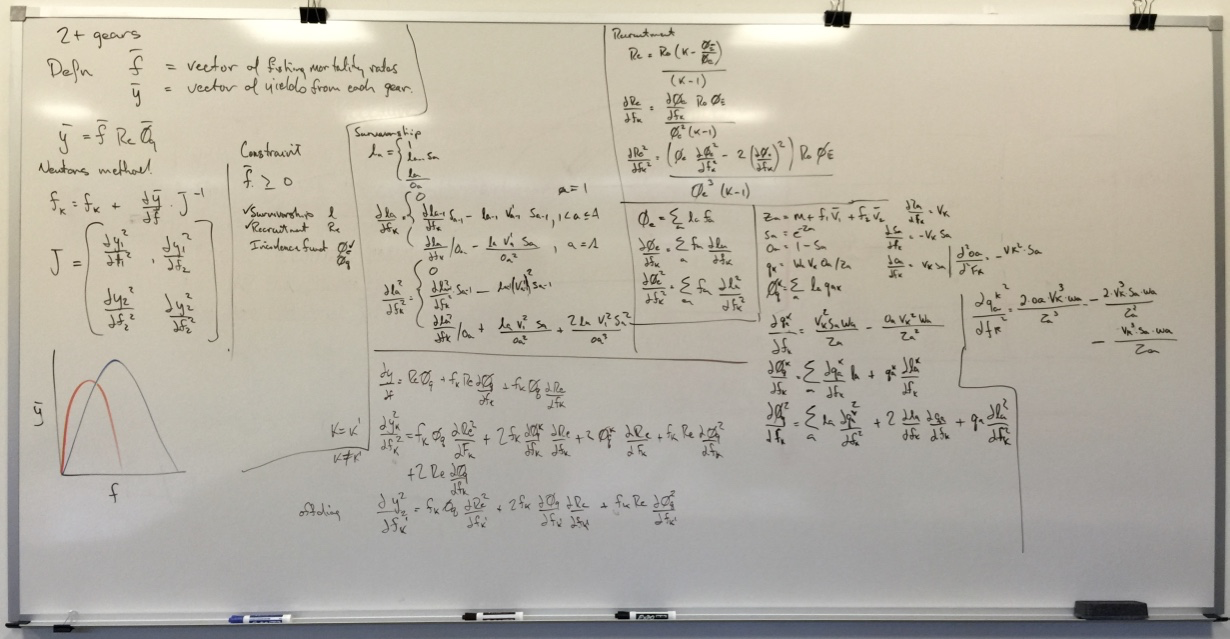
\includegraphics[width=0.95\linewidth,keepaspectratio=true]{./whiteBoard.png}}

% \end{columns}

\begin{columns}
	% 
	% CATCH EQUATIONS
	% 
	\column{0.33}
	\block{Catch Equation And Finding \fmsy}{
		Assuming all fisheries and natural mortality operate simultaneously, the equilibrium catch equation for each fleet can be written as a vector
		\begin{align}
			%
			\vec{y} = \vec{f} R_e \vec{\phi}  \label{eq.1}
			%
		\end{align}
		To find the vector of fishing mortality rates that simultaneously maximizes the yield for each fleet we use Newton's method to find the solution to $\dfrac{\partial \vec{y}}{\partial \vec{f}} = 0$.  The first and second derivatives of \eqref{eq.1} for fleet $k$ are given by:
		\begin{align}
			%
			\dye &= R_e \phi_k
			+ f_k R_e \dphi
			+ f_k \phi \dre \label{eq.2} \\[1ex] 
			%
			\mbox{Jacobian} \nonumber \\
			\ddye &=
			\begin{cases}
				f_k \phi \ddre + 2 f_k \dphi \dre + 2 \phi_k \dre + f_k R_e \ddphi + 2 R_e \dphi & k = k \\[2ex]
				%
				f_{k'} \phi \ddre + 2 f_{k'} \dphi \dre + f_{k'} R_e \ddphi & k \neq k'
			\end{cases} \label{eq.3}
		\end{align}
		The Newtons iteration step is given by:
		\begin{align}
			\vec{f}_{i+1} = \vec{f}_{i} - \dfrac{\partial y}{\partial f}
			 \left( \dfrac{{\partial y}^2}{{\partial f}^2} \right)^{-1} \label{eq.4}
		\end{align}
	}% end block.

	% 
	% MATH SYMBOLS USED IN EQUATIONS
	% 
	\note[
		width=11cm,
		targetoffsetx=-10.5cm,
		targetoffsety=-11cm,
		rotate=00,
		angle=0,
		radius=0cm,
		connection
		]
	{	
		\textbf{Symbols}\\
		\begin{tabular}{cl}
			$\vec{f}$     & fishing mortality rates.\\
			$\vec{y}$     & equilibrium yields.\\
			$\vec{\phi}$  & yield per recruit.\\
			$R_e $        & equiliibrium recruitment.\\
		\end{tabular}
	}

	% 
	% SURVIVORSHIP
	% 
	\column{0.33}
	\block{Survivorship}{
		The age-specific total mortality rate and survival rate is defined as \[ z_a = M_a + \sum_k f_k v_{k,a}, \quad s_a = \exp(-z_a).\]
		The survivorship of a chorot is based on the following recurstive function:
		\begin{align}
			l_a &= \begin{cases}
				1,  & a = 1\\[1ex]
				l_{a-1} s_{a-1}, & 1<a<A\\[1ex]
				\dfrac{l_{a}}{1 - s_{a}}, & a = A
			\end{cases}\label{eq.5} \\[1ex]
		\end{align}
		and the vectors of first and second derivatives are:
		\begin{align}
			\dla &= \begin{cases}
				0, & a=1\\[1ex]
				% 
				s_{a-1} \cdot\left(\dfrac{\partial l_{a-1}}{\partial f_k} - l_{a-1}v_{k,a-1} \right), & 1 < a < A\\[3ex]
				% 
				\dfrac{1}{\left(1-s_a \right)} \cdot
				\left[
					\dfrac{\partial l_{a}}{\partial f_k}
					 - \dfrac{{{l}_{a}} {{v}_{k,a}} { s_{a}} }
					{{{\left( 1-{s_{a}}\right) }}}
					\right], & a = A 
			\end{cases}\label{eq.7} \\[3ex]
			% 
			% 
			\ddla & = \begin{cases}
				0, & a = 1\\[1ex]
				%
				{ s_{a-1} }\cdot \left(
				\dfrac{{\partial^2 l_{a-1}}} {{\partial f_k}^2}
				+ {{l}_{a-1}} {{v}_{k,a-1}^{2}} 
				\right), & 1<a<A\\[3ex]
				%
				\dfrac{1}{\left(1-s_a \right)} \cdot
				\ddla \cdot \dfrac{ {{l}_{a}} {{v1}_{a}^{2}} {{s}_{a}} } 
				{ (1- s_a) }
				+
				\dfrac{ 2  {{l}_{a}}  {{v}_{k,a}^{2}}  {{s}_{a}}^2 } 
				      {(1-s_a)^3} & a = A
				% \dfrac{ {{l}_{a}} {{v}_{k,a}^{2}} }} {{{\left( 1-{{e}^{-m-{{v2}_{a}}\cdot f2-{{v1}_{a}}\cdot f1}}\right) }^{2}}}+\frac{2\cdot {{l}_{a}}\cdot {{v1}_{a}^{2}}\cdot {{e}^{-2\cdot m-2\cdot {{v2}_{a}}\cdot f2-2\cdot {{v1}_{a}}\cdot f1}}}{{{\left( 1-{{e}^{-m-{{v2}_{a}}\cdot f2-{{v1}_{a}}\cdot f1}}\right) }^{3}}}
			\end{cases} \label{eq.8}
		\end{align}
	}


\end{columns}
	\block{~}{
		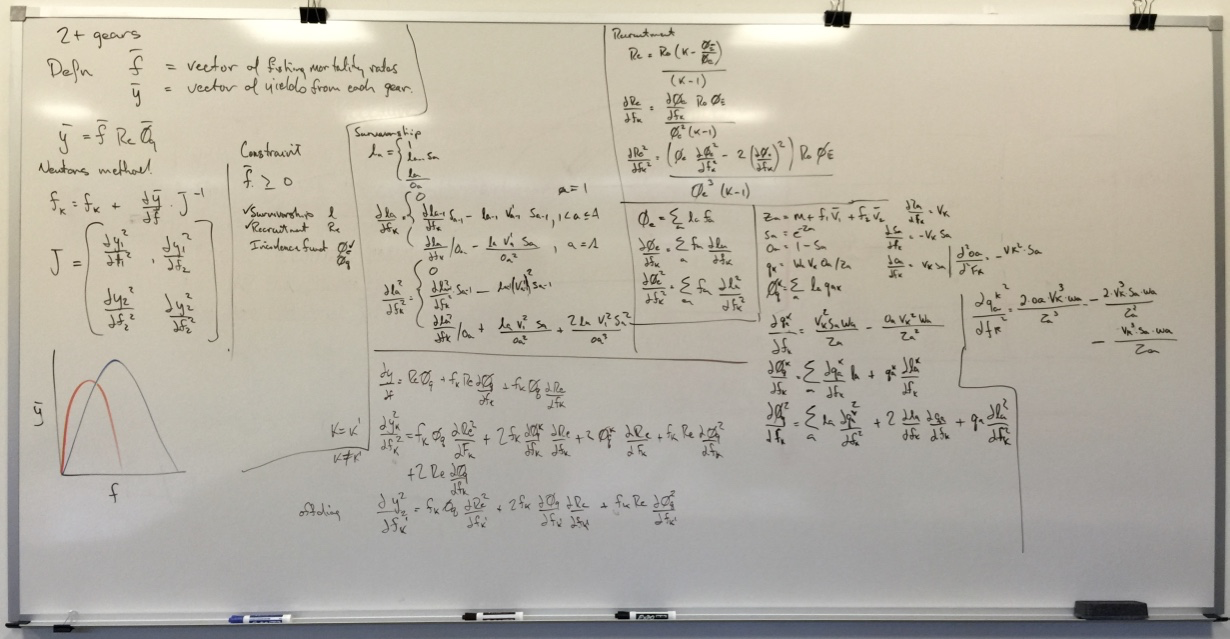
\includegraphics[width=0.95\linewidth,keepaspectratio=true]{./whiteBoard.png}
	}
	

\end{document}